\question{Уравнение движение электрона в неоднородном аксиально-симметричном
  магнитном поле}

Воспользуемся уравнением \( d\vec{p}/dt = \vec{F} \) и 
\( \vec{E} = q\vec{E} + q[\vec{v}\vec{B}] \) при условии \( E_0 = 0 \) и 
\( v \ll c \):
\begin{equation}
	m_0 \frac{d^2 \vec{r}}{dt^2} = q[\vec{v}\vec{B}_0]
	\label{eq11.2.47}
\end{equation}

Имеем выражения для индукции магнитного поля 
\[
	\begin{array}{c}
		B_{0z}(r,z) = \sum\limits_{n=0}^{\infty}(-1)^n 
			\frac{B_0^{(2n)}(z)}{(n!)^2}\left(\frac{r}{2}\right)^{2n}; \\
		B(r,z) = \sum\limits_{n=0}^{\infty}(-1)^{n+1} 
			\frac{B_0^{(2n+1)}(z)}{n!(n+1)!}\left(\frac{r}{2}\right)^{2n+1}.
	\end{array}
\]
записанные в цилиндрической системе координат, поэтому преобразуем декартовы 
координаты в цилиндрические:
\begin{equation}
	\left. \begin{array}{c}
		x = r\cos\phi \\
		y = r\sin\phi \\
		z = z
	\end{array} \right\}
	\label{eq11.2.48}
\end{equation}

Вектор лоренцевой силы \( \vec{F} = q[\vec{v}\vec{B}_0] \) имеет одно и то же 
направление и величину в любой системе координат. Тогда, если совместить оси 
\( 0z \) декартовой и цилиндрической системы координат, то значения радиальной 
\( F_r \) и азимутальной \( F_\phi \) -- составляющих силы можно просто 
получить по правилам преобразования систем координат при повороте их на 
некоторый угол \( \phi \) (рис.\ref{img11.1}):
\begin{equation}
	F_r = F_x \cos\phi + F_y \sin\phi, \quad
	F_\phi = -F_x \sin\phi + F_y \cos\phi
	\label{eq11.2.49}
\end{equation}
Здесь \( F_x = m_0 \ddot{x} \), \( F_y = m_0 \ddot{y} \). После подстановки в 
(\ref{eq11.2.49})  соответствующих производных по времени из 
(\ref{eq11.2.48}) находим:
\begin{equation}
	\left. \begin{array}{c}
		F_r = m_0 \left[ \ddot{r} - r(\dot{\phi})^2 \right] \\
		F_\phi = \frac{m_0}{r}\frac{d}{dt}\left( r^2\dot{\phi} \right)
	\end{array} \right\}
	\label{eq11.2.50}
\end{equation}

\begin{figure}[h!]
	\center
	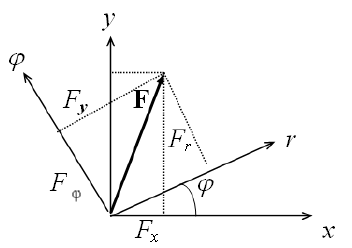
\includegraphics[width=.4\textwidth]{11_1}
	\caption{Преобразование систем координат}
	\label{img11.1}
\end{figure}

С учётом, что \( B_{0\phi} = 0 \) и что в цилиндрической системе координат 
\[
	[\vec{v}\vec{B}_0] = \left|
	\begin{array}{ccc}
		\vec{e}_r & \vec{e}_\phi & \vec{e}_z \\
		\dot{r}   & r\dot{\phi}  & \dot{z}   \\
		B_{0r}    & 0            & B_{0z}
	\end{array} \right|
\]
и из (\ref{eq11.2.47}) и (\ref{eq11.2.50}) получаем:
\begin{equation}
	\left. \begin{array}{c}
		m_0 \left[ \ddot{r} - r(\dot{\phi} \right] = qrB_{0z}\dot{\phi} \\
		\frac{m_0}{r}\frac{d}{dt}\left( r^2\dot{\phi} \right) = 
			q\left( -B_{0z}\dot{r} + B_{0r}\dot{z} \right) \\
		m_0 \ddot{z} = -qrB_{0r}\dot{\phi}
	\end{array} \right\}
	\label{eq11.2.51}
\end{equation}

Воспользуемся соотношением
\[
	B_{0z} = \frac{1}{r}\pder{}{r}\left( rA_\phi \right);\quad
	B_{0r} = -\pder{A_\phi}{z};\quad
	\pder{B_{0r}}{z} - \pder{B_{0z}}{r} = 0
\]
и выразим \( B_{0z} \) и \( B_{0r} \) через \( A_\phi \). В результате 
(\ref{eq11.2.51}) преобразуется к виду:
\begin{equation}
	\left. \begin{array}{c}
		m_0 \left[ \ddot{r} - r(\dot{\phi} \right] = 
			q\dot{\phi}\pder{rA_\phi}{r} \\
		\frac{m_0}{r}\frac{d}{dt}\left( r^2\dot{\phi} \right) = 
			q\left[ -\dot{z}\pder{A_\phi}{z} - 
			\frac{\dot{r}}{r}\pder{rA_\phi}{r} \right] \\
		m_0 \ddot{z} = -qr\dot{\phi}\pder{A_\phi}{z}
	\end{array} \right\}
	\label{eq11.2.52}
\end{equation}

Интегрируя второе уравнение системы (\ref{eq11.2.52}) по времени, находим
\begin{equation}
	\dot{\phi} = -\frac{q}{m}\frac{A_\phi}{r}
	\label{eq11.2.53}
\end{equation}
при условии, что при влёте в область, где существует магнитное поле, 
отсутствует азимутальная составляющая скорости 
\( \left. \dot{\phi} \right|_{t=0} = 0 \), 
\( \left. A_\phi \right|_{t=0} = 0 \).

В параксиальной области учтём только первый член в разложении 
\( A_\phi = \frac{r}{2} B_0(z)\). Тогда
\[
	\dot{\phi} = -\frac{q}{2m_0}B_0(z)
\]

Угол поворота траектории при движении частицы вдоль оси \( 0z \) можно 
вычислить, если учесть, что 
\[
	\dot{\phi} = \pder{\phi}{z}\frac{dz}{dt} = v_0 \pder{\phi}{z}
\]

Здесь \( v_0 \) -- скорость частицы, определяемая из условий сохранения 
энергии \( \frac{m_0 v_0^2}{2} = -qU_0 \), где под \( U_0 \) понимается 
потенциал, необходимый для придания частице скорости \( v_0 \) вдоль оси 
\( 0z \) на влёте в область существования поля. Тогда из (\ref{eq11.2.55}) 
имеем:
\[
	\pder{\phi}{z} = \sqrt{-\frac{q}{8m_0 U_0}} B_0(z)
\]
а угол поворота при движении частицы в магнитном поле от точки \( z_0 \) до 
точки \( z_1 \) равен:
\[
	\phi(z) = \sqrt{-\frac{q}{8m_0 U_0}} \int\limits_{z_0}^{z_1} B_0(z) dz
\]

Видно, что угол поворота не зависит от \( r_0 \) -- начального положения 
частицы, поэтому любая из одинаковых частиц, влетающих в точке \( z_0 \) при 
любых \( r_0 \) и \( \phi_0 \), повернётся на один и тот же угол. 

Знак минус под знаком радикала свидетельствует о том, что для отрицательно 
заряженный частиц (\( q < 0 \)) ускоряющим является положительный потенциал 
\( U_0 \), а для положительных заряженных частиц -- отрицательный, то есть в 
плоскости \( r_0 \) уравнение траектории получим, подставив решение 
(\ref{eq11.2.53}) в первое уравнение (\ref{eq11.2.52}):
\begin{equation}
	\ddot{r} - r\left( \frac{q}{m_0}\right)^2 \frac{A_\phi}{r^2} = 
		-\left( \frac{q}{m_0} \right)^2 \frac{A_\phi}{r}
		\left( A_\phi + r\pder{A_\phi}{r} \right)
	\label{eq11.2.58}
\end{equation}

В искомом приосевом приближении 
\( r\pder{A_\phi}{r} = \frac{r}{2} B_0(z) = A_\phi \) и (\ref{eq11.2.58}) 
приводится к виду
\[
	\ddot{r} = -\left( \frac{q}{m_0} \right)^2 \frac{r}{4} B_0^2(z)
\]
С учётом преобразования
\[
	\ddot{r} = \frac{d}{dz}\left( \frac{dr}{dz}\dot{z} \right)\dot{z} = 
		\frac{d^2 r}{dz^2}(\dot{z})^2 = -\frac{q}{m_0}2U_0\frac{d^2 r}{dz^2}
\]
получаем:
\[
	\frac{d^2 r}{dz^2} = \frac{q}{8m_0 U_0}rB_0^2(z)
\]